\chapter{Theoretischer Hintergrund}
\label{chap:technischerHintergrund}
In diesem Kapitel werden die technischen Hintergründe von \gls{open-ran} und O-Ran erläutert, und auf die technischen Implementierungen der \gls{foran}-Anwendungen eingegangen. Außerdem werden die \gls{mitre} Frameworks und Datenquellen für die empirische Analyse vorgestellt.

\section{Open RAN und O-RAN}
\label{sec:tech-openran}
Die \gls{open-ran} Architektur bietet eine innovative Möglichkeit, die traditionell monolithische Struktur der \gls{ran} (deutsch: Funkzugangsnetze) durch modulare und offene Ansätze zu ersetzen. Dieser Wandel wird vor allem durch die \orana{} und die O-RAN \gls{sc} vorangetrieben. Ziel ist es, die Interoperabilität zwischen verschiedenen Komponentenherstellern zu verbessern und neue Möglichkeiten für Automatisierung und Sicherheit zu schaffen.

\begin{figure}
    \centering
    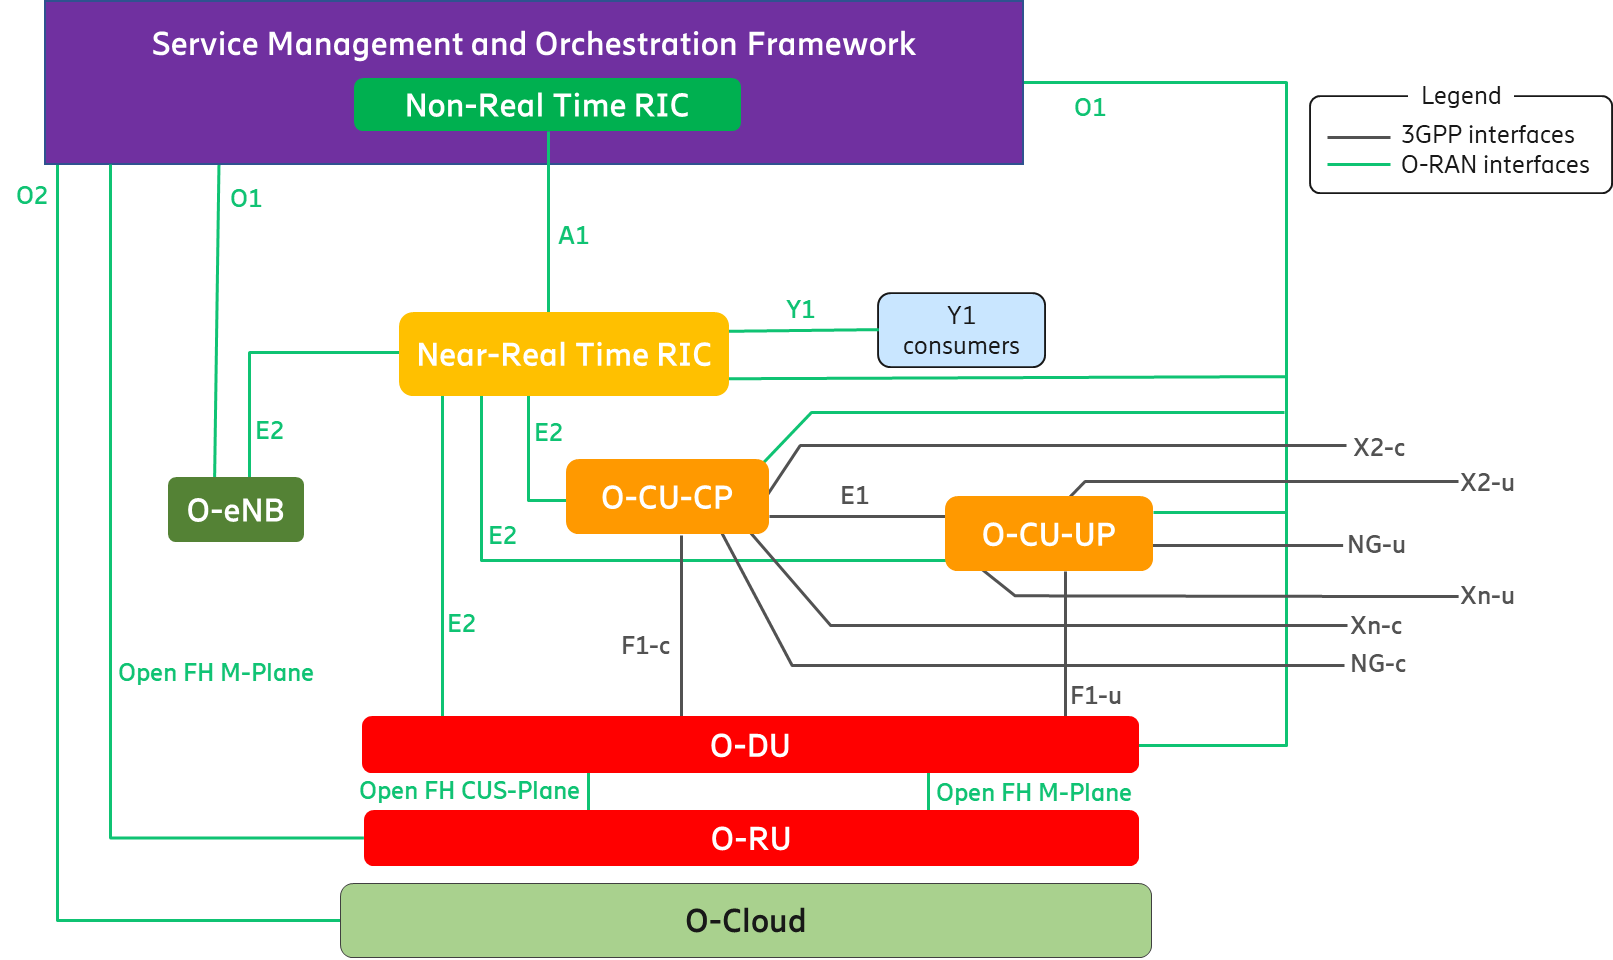
\includegraphics[width=0.6\textwidth]{oran-architecture}
    \caption{Logische Architektur von O-RAN (Quelle: \autocite{ORANAlliance})}
    \label{fig:oran-architecture}
\end{figure}

Die Architektur des O-RAN, dargestellt in Abbildung \ref{fig:oran-architecture}, wird von der \gls{wg1} verantwortet und in verschiedenen \textit{Task Groups} entwickelt. Sie basiert auf der Definition von standardisierten offenen Schnittstellen und einer logischen Trennung zwischen den Hauptfunktionen eines \glspl{ran}. Dazu gehören unter anderem der nicht-echtzeitfähige RAN-Intelligent-Controller (Non-RT-RIC) und der nahezu-echtzeitfähige RIC (Near-RT-RIC), die jeweils für unterschiedliche Steuerungszyklen optimiert sind \autocite{o-ranworkgroup1usecasesandoverallarchitectureORANArchitectureDescription2024}.

\section{Virtualisierung mit Kubernetes}
Die O-RAN \gls{sc} Referenzimplementierung basiert grundlegend auf Kubernetes, einer Plattform zur Orchestrierung von containerisierten Anwendungen \autocite{ReleaseReleasesConfluence}. Kubernetes ermöglicht es, Anwendungen in Containern auszuführen, die von ihrer Umgebung unabhängig sind und so eine hohe Flexibilität und Skalierbarkeit bieten. Container können durch Software wie Docker erstellt werden und nutzen Virtualisierung auf Betriebssystemebene, um eine isolierte Laufzeitumgebung für O-RAN Komponenten zu schaffen. Kubernetes orchestriert diese Container, indem es deren Bereitstellung, Skalierung und Verwaltung automatisiert. Das Konzept der Virtualisierung, auf dem Kubernetes aufbaut, hat zum Ziel, physische Ressourcen wie Prozessor und Arbeitsspeicher abstrahiert bereitzustellen. Dabei werden mehrere virtuelle Container auf einer physischen Maschine betrieben. Trotz der Vorteile bringt die Nutzung von Kubernetes und Virtualisierung auch Sicherheitsrisiken mit sich. Angriffsvektoren können durch falsch konfigurierte Container, ungesicherte Schnittstellen oder Schwachstellen in der Orchestrierungsplattform selbst entstehen.
\par Mit Ausnahme der O-RAN Radio Unit (O-RU) können alle Komponenten der Abbildung \ref{fig:oran-architecture} vollständig containerisiert, das heißt in einer virtuellen Umgebung ausgeführt, werden. Die O-RU ist die hardware-nächste Komponente und benötigt spezialisierte Hardware zur Verarbeitung der empfangenden Signale.

\section{5G-FORAN}
\label{sec:tech-foran}
Für das ATTACK-Teilvorhaben wurde ein Framework implementiert, das es ermöglicht Angriffe auf die implementierte \gls{open-ran} Infrastruktur auszuführen. Dazu können verschiedene Tools genutzt werden, solange sie über eine \gls{cli} verfügen. Das \gls{at} kann über diese Tools komplexe Angriffe simulieren und die Metadaten sowie Ergebnisse der Angriffe abspeichern. Zur Speicherung wird eine MongoDB Datenbank genutzt. MongoDB ist eine \textit{NoSQL}, dokumentenbasierte Datenbank \autocite{MongoDBDeveloperData}. Ein Dokument stellt im Kontext des \glspl{at} ein Artefakt dar, welches alle relevanten Informationen über einen Angriff enthält. Diese Datenbank ist die Basis für alle Abfragen und Visualisierungen, die über das Dashboard möglich sind.

\section{Dashboard}
\label{sec:tech-dashboard}
Das Dashboard ist ein Visualisierungtool, über das die Gesamtmenge aller Angriffssimulationen dargestellt werden kann. Für jeden Angriff werden die Metadaten und Ergebnisse textuell aufbereitet dargestellt und mit weiteren grafischen Visualisierungen, wie einem zeitlichen Verlauf, aufgewertet.
Das Dashboard ist über einen Webserver in der Programmiersprache \textit{Go} implementiert, der serverseitig eine Darstellung der Webseite erstellt und diese beim Aufruf der spezifischen Seiten des Dashboards an den Browser des Anwenders schickt. Neben den \gls{html} Dateien werden außerdem \gls{css} und \gls{js} Dateien ausgeliefert, welche die Weboberfläche stilisieren und Funktionalität hinzufügen, die nicht in \gls{html} ausgedrückt werden kann. Die Architektur des Dashboards basiert auf dem Hotwire (HTML-over-the-wire) Web-Framework, welches es zum Ziel hat, möglichst wenig \gls{js} im Frontend einzusetzen. Stattdessen werden \gls{html} Dateien dynamisch vom Server angepasst und in wenigen Millisekunden an den Client versandt. Dieser Ansatz ist weit verbreitet und wird auch als \textit{server-sided rendering} bezeichnet \autocite{HTMLWireHotwire}. Die einzelnen Seiten, die im Dashboard aufgerufen werden können, sind in einer Übersicht in Kapitel \ref{chap:implementierung} aufgelistet.
\par Diese Arbeit umfasst die Weiterentwicklung des Dashboards auf Basis einer vorangegangenen Forschungsarbeit für die Evaluation von Dashboardtechniken und der Implementierung eines Prototypen \autocite{weberEvaluationDashboardTechniques}.

\label{bg:mitre-frameworks}
\section{MITRE Frameworks}
\glsreset{mitre}
Die von der \gls{mitre}\footnote{Entgegen einem verbreiteten Missverständnis (ChatGPT-4 liegt auch falsch) steht MITRE \textbf{nicht} für "Massachusetts Institute of Technology Research and Engineering".} zur Verfügung gestellten Werkzeuge und Kategorisierungssysteme wurden entwickelt, um Sicherheitsrisiken zu analysieren, bewerten und behandeln. Die im Folgenden beschriebenen Frameworks bieten strukturierte Daten zur Analyse von Schwachstellen, Schwachstellenkategorien und Angriffsmustern. In diesem Kapitel werden die einzelnen Frameworks beschrieben und deren Anwendungsgebiete erläutert.

\subsection{MITRE ATT\&CK}
\glsreset{attack}
Das \gls{mitre} \gls{attack} Framework ist ein Wissensfundus, der Angriffstaktiken und -techniken dokumentiert, die auf realen Beobachtungen basieren. Es bietet eine strukturierte Möglichkeit, Angriffsmethoden zu analysieren und deren Auswirkung auf einzelne Systeme oder Infrastrukturen zu bewerten. In der aktuellen Version 16.1 enthält das Framework 14 Taktiken und 203 Techniken in der \textit{enterprise}-Matrix. Die Quelle ist aufgrund ihrer breiten Akzeptanz und der kontinuierlichen Aktualisierung durch die \gls{mitre}-Organisation als äußerst verlässlich einzustufen \autocite{MITREATTCK}. Es existieren diverse Spezialisierung der \gls{attack} Matrix, die sich auf konkrete Anwendungsfälle konzentrieren, wie zum Beispiel die \gls{mitre} \gls{atlas} Matrix. Diese beschäftigt sich insbesondere mit Angriffen auf KI-gestützte Systeme \autocite{ATLASMatrixMITRE}.

\subsection{CVE}
\label{bg:cve}
\glsreset{cve}
Das \gls{cve}-System ist eine standardisierte Referenzdatenbank, die bekannte Schwachstellen und Sicherheitslücken in Software und Hardware dokumentiert. Jeder \gls{cve}-Eintrag enthält spezifische Informationen zu einer identifizierten Schwachstelle und bietet eine Grundlage für die Kommunikation und Priorisierung von Sicherheitsmaßnahmen, darunter die folgenden Hauptbestandteile, die für diese Arbeit besonders relevant sind:

\begin{itemize}
    \item \textbf{CVE-ID}: Eine weltweit eindeutige Kennung im Format \texttt{CVE-JJJJ-NNNNN}, die die Schwachstelle klar identifiziert.
    \item \textbf{Betroffene Produkte}: Angaben zu spezifischen Softwareversionen oder Hardware, die von der Schwachstelle betroffen sind.
    \item \textbf{Schweregrad und CVSS-Wertung}: Integration mit dem \gls{cvss} das, neben anderen Metriken, eine Basisbewertung von 0 bis 10 bereitstellt, um die kritische Bedeutung der Schwachstelle zu quantifizieren.
    \item \textbf{Verknüpfungen zu CWE}: Hinweise auf zugrunde liegende Schwachstellen aus der \gls{cwe}-Taxonomie.
\end{itemize}

\subsection{CWE}
\label{bg:cwe}
\glsreset{cwe}
Die \gls{cwe} ist eine Aufzählung von häufigen Schwachstellenkategorien und Fehlermustern in Software und Hardware, die dazu dient, Sicherheitsprobleme systematisch zu identifizieren und zu dokumentieren \autocite{CWEWebsite}. Jede \gls{cwe}-Instanz beschreibt eine spezifische Schwachstellenkategorie, darunter die folgenden Hauptbestandteile, die für diese Arbeit besonders relevant sind:

\begin{itemize}
    \item \textbf{Schwachstellen-ID und Name}: Eine eindeutige Kennung und Beschreibung der Schwachstellenkategorie.
    \item \textbf{Übliche Konsequenzen}: Eine Liste von typischen Auswirkungen, die durch Ausnutzung einer Schwachstelle dieser Kategorie verursacht werden können.
    \item \textbf{Beobachtete Beispiele}: Verweise auf reale Anwendungsfälle, in denen ein \gls{cve} aus dieser Kategorie ausgenutzt wurde.
    \item \textbf{Demonstrative Beispiele}: Codebeispiele, die die Ausnutzung einer Schwachstelle dieser Kategorie illustrieren und deren Auswirkungen verdeutlichen.
\end{itemize}

\subsection{CAPEC}
\label{bg:capec}
\glsreset{capec}
Das \gls{capec} Framework zielt darauf ab, Angriffsmuster systematisch zu dokumentieren und zu klassifizieren, um Sicherheitsforscher:innen und Entwickler:innen bei der Identifikation und Vermeidung von Schwachstellen zu unterstützen. Jede \gls{capec}-Instanz beschreibt ein spezifisches Angriffsmuster, darunter die folgenden Hauptbestandteile, die für diese Arbeit besonders relevant sind:

\begin{itemize}
    \item \textbf{Angriffsmuster-ID und Name}: Eine eindeutige Kennung und Bezeichnung, die das Angriffsmuster klar identifiziert.
    \item \textbf{Beschreibung}: Eine kurze Beschreibung des Angriffs, seine Ziele und seinen Kontext.
    \item \textbf{Schwachstellenverknüpfungen}: Verweise auf relevante \glspl{cwe}, die die zugrunde liegenden Schwachstellen beschreiben, die der Angriff ausnutzt.
    \item \textbf{Taxonomie-Zuordnungen}: Verweise auf Objekte des \gls{attack} Frameworks
\end{itemize}

Die Datenbank ist umfassend und bietet eine hierarchische Klassifikation der Angriffsmuster, die es ermöglicht, zwischen allgemeinen Kategorien und spezifischen Instanzen zu navigieren. Diese Daten sind in der Sicherheitsforschung nützlich, da sie dabei helfen, typische Bedrohungen zu gruppieren und Szenarien für Sicherheitsüberprüfungen zu erstellen \autocite{CAPECWebsite}.

\par Das \gls{cve}-System unterscheidet sich von \gls{cwe} dadurch, dass es konkrete Sicherheitslücken in spezifischen Produkten beschreibt, während \gls{cwe} die allgemeine Kategorie oder Art der Schwachstelle adressiert. In Kombination mit der \gls{capec} und der \gls{cwe} ermöglicht die \gls{cve} eine ganzheitliche Analyse, die sowohl Schwachstellenursachen als auch deren Ausnutzung und Abwehrmaßnahmen abdeckt. Diese Eigenschaften machen die \gls{cve} zu einem unverzichtbaren Werkzeug in der Sicherheitsanalyse und ist auch sehr gut auf \gls{open-ran} Umgebungen anwendbar \cite{CVEWebsite}.

\section{Datenquellen}
\label{sec:datenquellen}
Die Integration von relevanten Datenquellen stellt eine wesentliche Grundlage für eine wissenschaftliche Sicherheitsanalyse dar. In diesem Kapitel werden Datenquellen beschrieben, die für diese Arbeit eine wichtige Rolle spielen.
\subsection{Bedrohungsmatrizen}
\par Die \gls{tm4k}, bereitgestellt von Microsoft, ist eine spezialisierte Threat-Matrix für Kubernetes-Umgebungen, die verschiedene Angriffsvektoren und Schwachstellen in containerisierten Plattformen kategorisiert. Sie enthält detaillierte Informationen zu typischen Angriffstechniken, Taktiken und entsprechenden Verteidigungsmaßnahmen, die speziell für Kubernetes relevant sind \autocite{TacticsThreatMatrix}. Die \gls{tm4k} stellt damit eine Spezialisierung der \gls{mitre} \gls{attack} dar, die auf den speziellen Anwendungsfall Kubernetes erstellt wurde. Die Quelle wurde seit der Erstveröffentlichung 2020 bis Anfang 2023 regelmäßig aktualisiert, hat aber seitdem keine Updates mehr bekommen, wird dennoch häufig genutzt und bietet eine hilfreiche Wissensquelle über die Angriffstechniken im Kubernetes Umfeld \autocite{DeploymentsMicrosoftThreatMatrixforKubernetes}. Eine erweitere Version der \gls{tm4k} ist die Redguard \gls{ktm}. Sie legt einen besonderen Fokus auf spezifische Angriffe und gibt für viele Techniken Kubernetes Manifeste und \gls{cli} Kommandos an, mit denen das eigene System auf die jeweilige Schwachstelle getestet werden kann. Ihre Anwendung in der Schwachstellenanalyse von O-RAN kann hilfreich sein, da sie spezifische Ressourcen für das Finden von Schwachstellen im System enthält \autocite{KubernetesThreatMatrix}. Die in dieser Matrix gelisteten Kommandos werden im \gls{at} genutzt, um das \textit{Kubernetes-Testing} auszuführen. Dafür kommt kein spezielles Tool zum Einsatz, sondern die Angriffe werden direkt über die Kubernetes \gls{cli} \verb|kubectl| ausgeführt.
\par Eine dritte Kategorisierung für Techniken stammt aus dem Report der \orana{} \gls{wg11}. Insgesamt identifiziert diese Risikoanalyse 104 Bedrohungen, die sich gegen die Komponenten eines O-RAN Systems inklusive der O-Cloud Komponente wenden (vgl. Abbildung \ref{fig:oran-architecture}) \autocite{o-ranworkgroup11securityworkgroupORANSecurityThreat2024}. Für jede dieser Bedrohungen wird eine \textit{Threat-ID} vergeben. Aufgrund des sehr speziellen Anwendungsfalls werden in dem Report Bedrohungen beleuchtet, die nicht in der \gls{tm4k} oder \gls{ktm} abgebildet sind. Bisher sind die im \gls{at} implementierten Angriffe jedoch nicht so sehr spezialisiert, sodass eine Zuordnung zu einer Technik aus einer der anderen Matrizen immer möglich ist.
\subsection{Datenquellen für empirische Analyse}
\par In der Implementierung von \gls{acema} werden Daten aus externen Datenquellen genutzt. Für das Mapping von \gls{mitre}-Technik zu \gls{cve} wird das \gls{mitre}-\gls{cti} Repository genutzt. Weitere Informationen über einen spezifischen \gls{cve} werden über die \gls{nvd} des \gls{nist} beschafft.
\par Das \gls{cti} Repository enthält eine Vielzahl an Daten zur Identifikation und Kategorisierung von Cyberangriffstechniken. Es stellt spezifische Zuordnungen zwischen den im \gls{mitre} \gls{attack}-Framework beschriebenen Angriffstechniken und Schwachstellen (\glspl{cwe}) bereit, die eine wichtige Grundlage für Bedrohungsanalysen bilden. Diese Informationen umfassen unter anderem Angriffsmethoden, Exploit-Beschreibungen und potenzielle Abwehrmaßnahmen. Wissenschaftlich anerkannt ist das Repository durch die breite Akzeptanz des \gls{mitre} \gls{attack}-Frameworks in der Sicherheitsforschung sowie durch die Anwendung in praxisorientierten Sicherheitslösungen.
\par Die \gls{nvd} ist eine zentrale Datenbank des \gls{nist}, die umfassende Informationen zu Schwachstellen und deren Bewertungen liefert. Sie basiert auf international anerkannten Standards wie \gls{cve} und \gls{cvss}, um die Schwere und Ausnutzbarkeit von Sicherheitslücken zu quantifizieren. Die \gls{nvd} ist aufgrund der Bereitstellung standardisierter Sicherheitsmetriken ein unverzichtbares Werkzeug in der Sicherheitsforschung. Die Kombination aus systematischer Datenaufbereitung und fundierten Bewertungen macht die \gls{nvd} besonders geeignet für die Implementierung von Sicherheitslösungen und lässt sich standardmäßig in viele Management- und Dokumentationslösungen in Enterprise Umgebungen integriert \autocite{AssetsNVDIntegration,InformationenNVDIntegrationen}.